% Finished July 18, 2013
% Put into format of VUW Thesis on March 20, 2014.

\documentclass[12pt, a4paper, twoside, openright]{book}

\usepackage{vuwthesis} % sets up some local things, mostly the front page

\setlength{\intextsep}{12pt} % set space above and below in-line float
\setlength{\abovecaptionskip}{0pt} % set space between figure and caption.


\usepackage{amssymb, amsmath}
%\usepackage{mathtools}
\usepackage{tikz}
\usetikzlibrary{calc}

\newcommand{\beff}{\ensuremath{b_{\mathrm{eff}}}}
\newcommand{\bhom}{\ensuremath{b_{\mathrm{hom}}}}
\newcommand{\bmin}{\ensuremath{b_{\mathrm{min}}}}


%\usepackage{marvosym}

\usepackage{etoolbox}
\newtoggle{compilealone}
\toggletrue{compilealone}

\title{Chapter 6: The Homogenized Effective Slip Length}
\author{Nat Lund}

\begin{document}
\chapter{The Homogenized Effective Slip Length}\label{C:homog}

In this chapter, we shall find the \emph{homogenized slip length} of a bulk of fluid flowing over a rough slippery surface.  We start by giving a high-level overview of the homogenization technique, then explain each aspect of homogenization in detail.  The first aspect we explain is the variational formulation and its relation to the calculus of variations.  Then the Stokes equations are put into variational form, then we find the variational formulation of the Stokes equation with the full tensor slip boundary condition.  We then take a step sideways and tackle the concept of weak convergence, and show that periodic functions weakly converge to their mean.  With all the machinery finally in place, we homogenize the variational formulation of the Stokes equation with tensor slip.  From the homogenized formulation, we derive the homogenized effective slip length.  We close the chapter with discussion of the physical interpretation of the result and its likely range of applicability.

\clearpage
In our mathematical model of the system, fluid flow at each point in the bulk obeys Stokes equation:
\begin{equation}
\mu \nabla^2 \vec{u} = \nabla p
\end{equation}
And fluid at each point on the boundary satisfies the generalized slip boundary condition:
\begin{equation}
\vec{u} = b \, (\nabla \vec{u} + \nabla \vec{u}^T) \cdot \vec{n}
\end{equation}

%The boundary itself roughly coincides with the $x,y$ plane. 
The boundary is a surface described by a periodic height function $h(x,y)$ on the $x,y$ plane.  $h(x,y)$ may be defined so that the $z=0$ plane is at the tops of the peaks of $h(x,y)$.  
%The $z$ direction is roughly perpendicular to the boundary, and 
The fluid may be supposed to be flowing in the $x$ direction. The model is summarized in Figure (\ref{homogmodel}).

\begin{figure}[ht]
\centering
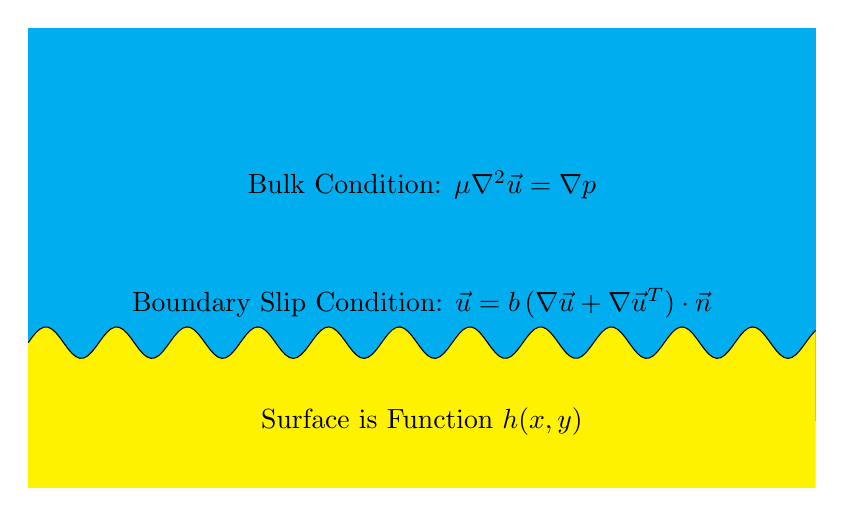
\begin{tikzpicture}
\fill[color=cyan] (0,-1) rectangle (10,4);

\node at (5,2) {Bulk Condition: $\mu \nabla^2 \vec{u} = \nabla p$};
\node at (5,0.5){Boundary Slip Condition:  $\vec{u} = b \, (\nabla \vec{u} + \nabla \vec{u}^T) \cdot \vec{n}$};

\fill [color=yellow,domain=0:10,samples=200] plot (\x,{ 0.2 * sin(7*\x r)} ) -- ++(0,-2) -| (0,0);
\draw [domain=0:10,samples=200] plot (\x,{ 0.2 * sin(7*\x r)} );

\node at (5,-1) {Surface is Function $h(x,y)$};

\end{tikzpicture}
\caption{Summary of the mathematical model.}\label{homogmodel}
\end{figure}

The \emph{effective} slip length of a rough surface was defined back in Chapter 1.  At sufficient height above the surface, perturbations due to the rough surface have died away, and the flow \emph{behaves like} flow in an \emph{effective system:} flow over a flat `effective' surface with a uniform slip length, $\beff$. We illustrate this with Couette-type flow in Figure (\ref{Couettelike}).

\begin{figure}[ht]
\centering
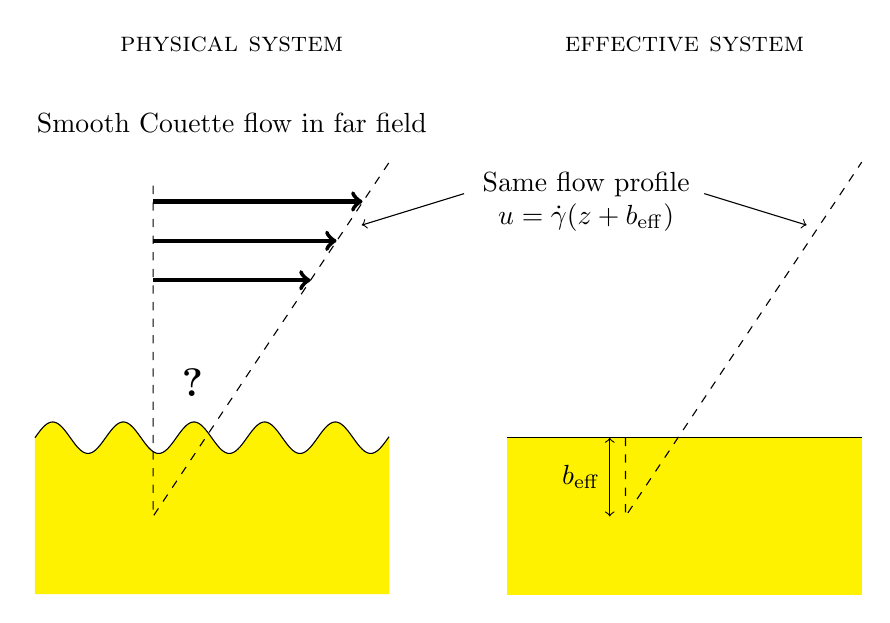
\begin{tikzpicture}

\coordinate (ori) at (0,0);
%\fill[color=cyan] (ori) ++(0,-1) rectangle ++(4.5,5);
\fill [color=yellow,domain=0:4.5,samples=200] plot (\x,{ 0.2 * sin(7*\x r)} ) -- ++(0,-2) -| (ori);
\draw [domain=0:4.5,samples=200] plot (\x,{ 0.2 * sin(7*\x r)} );

\draw[dashed] (ori) ++(1.5,3.2) -- ++(0,-4.2) -- ++(3,4.5);
\draw[->, ultra thick] (ori) ++(1.5,2) -- ++(2,0);
\draw[->, ultra thick] (ori) ++(1.5,2.5) -- ++(2.33,0);
\draw[->, ultra thick] (ori) ++(1.5,3) -- ++(2.66,0);
\node at (2,0.7) {\Large{\textbf{?}}};
\node at (2.5,4) {Smooth Couette flow in far field};


\coordinate (ori) at (6,0);
%\fill[color=cyan] (ori) ++(0,-1) rectangle ++(4.5,5);
\fill[color=yellow] (ori) rectangle ++(4.5,-2);
\draw (ori) -- ++(4.5,0);

\draw[dashed] (ori) ++(1.5,0) -- ++(0,-1) -- ++(3,4.5);
\draw[<->] (ori) ++(1.3,0) -- node[left] {\beff} ++(0,-1);

\draw[<-] (4.15,2.7) -- ++(1.3,0.4);
\draw[<-] (9.8,2.7) -- ++(-1.3,0.4);
\node at (7,3) [align=center] {Same flow profile\\$u = \dot{\gamma} (z + \beff)$};

\node at (2.5,5) {\textsc{physical system}};
\node at (8.25,5) {\textsc{effective system}};


\end{tikzpicture}
\caption{The effective slip length of Couette-type flow.}\label{Couettelike}
\end{figure}


\subsection{Homogenization}

Homogenization is a modern technique for approximating the solutions of partial differential equations, developed in the 1960s and '70s.  It began with the study of PDEs with rapidly oscillating coefficients.  
The basic idea was to identify the period of oscillation with a small parameter $\epsilon$, and to consider the limit as the period tended to zero.  Depending on the problem, one may get a solution as a series in $\epsilon$: $u = u_0 + \epsilon u_1 + \cdots$, or one may obtain a limiting PDE for which a solution can be found.
The technique can be applied to PDEs that hold on periodic structure; $\epsilon$ is the period of the structure.  Then we find an `effective' structure as the period of the structure tends to zero.  The first book describing homogenization appeared in 1978: ``Asymptotic Analysis for Periodic Structure", by Alain Bensoussan, Jacques-Louis Lions and George Papanicolaou.  

In standard homogenization techniques, it turns out to be necessary to cast the differential equations into variational or integral form.  As a consequence, in some cases it may be possible to exploit the fact that periodic functions weakly converge to their average.  (Weak convergence --- a `convergence under the integral sign' --- will be defined shortly.)
The homogenized solution is an approximation to the solution for a system with a finite period.  The smaller the period, the better the approximation.



\vspace{1em}
Thus, homogenization is perfectly suited to our task.  
In order to use homogenization, we must slightly extend our mathematical model with the following assumptions:

\vspace{1em}
First of all, we must assume that our surface roughness is \textbf{periodic}.  That is, $h(x,y)$ is a periodic function.  This is reasonable, many real rough surfaces are at least quasi-periodic; there seems no loss of information by assuming that the surface is periodic.

Secondly, we must assume the the intrinsic slip length is a periodic function with the \textbf{same period as the roughness}. % Again, this is reasonable.   
This is applicable in many situations -- though there may be interesting exceptions -- since
in many physical systems, the change in intrinsic slip length is \emph{due to} the roughness, eg. the increased slip over nanobubbles.

\vspace{1em}
Then, broadly speaking, the homogenization procedure is as follows:
The period is reduced sequentially, eg. the period is halved at each step in a sequence.
The \emph{amplitude} of the roughness must be reduced at the same rate, so that local gradient and curvature of the surface remain unchanged.  In the limit of the period tending to zero, we have the \textbf{homogenized} equations of flow, which we can consider to model a homogenized system.  The homogenized equations contain a slip length parameter.  In the language of homogenization theory, this is known as the \textbf{effective} slip length parameter.
We  illustrate this with Couette-type flow in Figure (\ref{Couettehomog}).

\begin{figure}[ht]
\centering
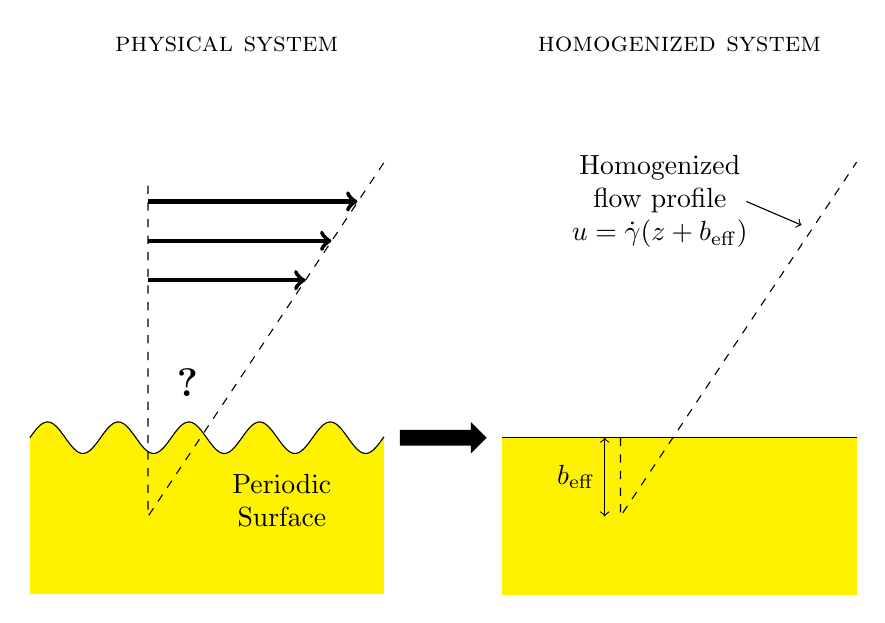
\begin{tikzpicture}

\coordinate (ori) at (0,0);
%\fill[color=cyan] (ori) ++(0,-1) rectangle ++(4.5,5);
\fill [color=yellow,domain=0:4.5,samples=200] plot (\x,{ 0.2 * sin(7*\x r)} ) -- ++(0,-2) -| (ori);
\draw [domain=0:4.5,samples=200] plot (\x,{ 0.2 * sin(7*\x r)} );

\draw[dashed] (ori) ++(1.5,3.2) -- ++(0,-4.2) -- ++(3,4.5);
\draw[->, ultra thick] (ori) ++(1.5,2) -- ++(2,0);
\draw[->, ultra thick] (ori) ++(1.5,2.5) -- ++(2.33,0);
\draw[->, ultra thick] (ori) ++(1.5,3) -- ++(2.66,0);
\node at (2,0.7) {\Large{\textbf{?}}};
\node at (3.2,-0.8)[align=center] {Periodic\\ Surface};


\coordinate (ori) at (6,0);
%\fill[color=cyan] (ori) ++(0,-1) rectangle ++(4.5,5);
\fill[color=yellow] (ori) rectangle ++(4.5,-2);
\draw (ori) -- ++(4.5,0);

\draw[dashed] (ori) ++(1.5,0) -- ++(0,-1) -- ++(3,4.5);
\draw[<->] (ori) ++(1.3,0) -- node[left] {\beff} ++(0,-1);

\draw[<-] (9.8,2.7) -- ++(-0.7,0.3);
\node at (8,3) [align=center] {Homogenized\\ flow profile\\$u = \dot{\gamma}( z + \beff)$};

\node at (2.5,5) {\textsc{physical system}};
\node at (8.25,5) {\textsc{homogenized system}};

\fill (5.8,0) -- ++(-0.2,0.2) -- ++(0,-0.1) --++(-0.9,0) -- ++(0,-0.2) -- ++(0.9,0) -- ++(0,-0.1);

\end{tikzpicture}
\caption{The homogenized effective slip length of Couette-type flow.}\label{Couettehomog}
\end{figure}

For Couette-type flow, we have defined the effective slip length as the slip length of an `effective' physical system, with flow solution $u = \dot{\gamma} (z + \beff)$.

If the same system is homogenized, the solution to the homogenized equations is $u = \dot{\gamma} (z + \beff)$.  We see immediately that the homogenized effective slip length exactly matches our physical definition of effective slip length.

\vspace{1em}
Let us now homogenize the Stokes equations for flow over rough periodic surfaces with variations in slip of the same period.  The particular homogenization technique we shall use comprises the following steps:

\subsubsection{Homogenization Process Overview}

\begin{enumerate}
\item Convert the model PDEs to variational (integral) form.
\item Create a sequence of variational formulations.
\item Find the limit formulation of the sequence:
\begin{itemize}
    \item Periodic functions weakly converge to their mean;
    \item This lets us find the limit formulation.
\end{itemize}
      
\item Convert the limit formulation back to classical formulation
\item Extract the implied slip length as the \emph{homogenized} slip length.
\end{enumerate}



\section{Variational Form}

The variational form comes originally from the Calculus of Variations.  The canonical use for the calculus of variations is with a \emph{minimization} problem.  We seek a \emph{function} on a domain that minimizes some quantity.  The quantity to be minimized is a \emph{functional}, a mapping from the space of functions to the real numbers.  The functional will be some kind of integral, with the integrand being some combination of the function, its derivatives (of various order), and position in the domain.

\begin{equation}
F(u) = \int_a^b f(u,u', ...\, ,x) \; dx,  \qquad F(u) \mapsto \mathbb{R}
\end{equation} 

The boundary values of the function $u(x)$ are given.  The basic concept of calculus of variations is to take $u(x)$ to be the solution function that minimizes the functional $F$.  That being the case, any \emph{variation} away from $u$, however small, will increase $F$.  Let $v(x)$ be an arbitrary function that is zero at the boundary (i.e. zero at $a$ and $b$), and let $\epsilon$ be a small parameter. Then:
\begin{equation}
F(u) \leq F(u + \epsilon v) \qquad \forall v: v(a) = v(b) = 0
\end{equation}
This minimizing function and variation are depicted in Figure (\ref{variation_c}).

\begin{figure}[ht]
\centering
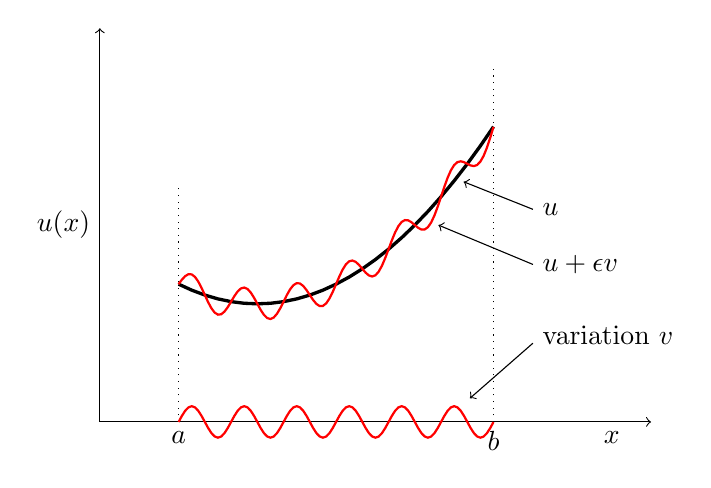
\begin{tikzpicture}

\draw[<->] (7,0) -- (0,0) -- node[left]{$u(x)$} (0,5);
\node at (6.5,0) [below] {$x$};
\draw[dotted] (1,0) -- +(0,3);
\draw[dotted] (5,0) -- +(0,4.5);
\node at (1,0)[below] {$a$};
\node at (5,0)[below] {$b$};

%\draw[very thick] (1,2) to [out=-50, in=180] (2,1.5) to [out=0,in=240] (5,3.5);
\draw[very thick, domain=1:5] plot (\x, { 1.5 + 0.25*(\x-2)*(\x-2) });
\draw[color=red,thick, samples=97, domain=1:5] plot (\x, { 0.2 * sin( 3*pi*(\x-1) r) } );
\draw[color=red,thick, samples=97, domain=1:5] plot (\x, { 1.5 + 0.25*(\x-2)*(\x-2) + 0.2 * sin( 3*pi*(\x-1) r)  });

\draw[<-](4.7,0.3) -- (5.5,1);
\node at (5.5,1.1)[right] {variation $v$};
\draw[<-] (4.62,3.05) -- (5.5,2.7);
\node at (5.5,2.7)[right] {$u$};
\draw[<-] (4.3,2.5) -- (5.5,2);
\node at (5.5,2)[right] {$u + \epsilon v$};

\end{tikzpicture}
\caption{The minimizing function $u(x)$ and an arbitrary variation $v(x)$ added to it.}\label{variation_c}
\end{figure}

For an arbitrary variation $v$, the small parameter $\epsilon$ can be treated as a variable, so that $F(u + \epsilon v)$ is a function from $\mathbb{R}$ to $\mathbb{R}$. Since $u$ minimizes $F$, $\epsilon = 0$ minimizes $F(\epsilon): \mathbb{R} \mapsto \mathbb{R}$. % Here's the cunning bit: 
The minimum is a stationary point, so the \emph{slope} of $F(\epsilon)$ is zero also at the minimum.  That is, for minimizing function $u$, for any variation $v$,

\begin{equation}
\frac{d}{d \epsilon} F(u + \epsilon v) = 0
\end{equation}
This is shown in Figure (\ref{minimum_c}).

\begin{figure}[ht]
\centering
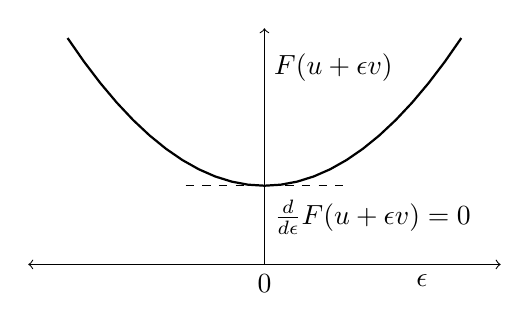
\begin{tikzpicture}
\draw[<->] ( -3,0) -- (3,0);
\draw[->] (0,0) --  (0,3);
\node at (2,0) [below] {$\epsilon$};
\node at (0,0) [below] {0};
\node at (0,2.5)[right]{$F(u + \epsilon v) $};

%\draw[thick,dashed] (-2.5,3) to [out=-60, in=180] (0,1) to [out=0, in=240] (2.5,3);
\draw[thick, domain=-2.5:2.5] plot ( \x, {1 + 0.3* \x*\x} );

\draw[dashed] (-1,1) -- +(2,0);
\node at (0,0.6) [right] {$\frac{d}{d \epsilon} F(u + \epsilon v) = 0$};
 
\end{tikzpicture}
\caption{The slope of $F(\epsilon)$ is zero at the minimum of $F(\epsilon)$.}\label{minimum_c}
\end{figure}


\subsection{Example: Energy Balance}

The fully-worked standard example of energy balance appears in Appendix D.  We give a summary here.

Consider a film of soapy water suspended across an aperture.  At equilibrium, the soap film lies in the $x,y$ plane.  Let $u(x,y)$ be the the height of the film above the $x,y$ plane (at point ($x,y$)), as in the schematic of Figure (\ref{soapy_c}).

\begin{figure}[ht]
\centering
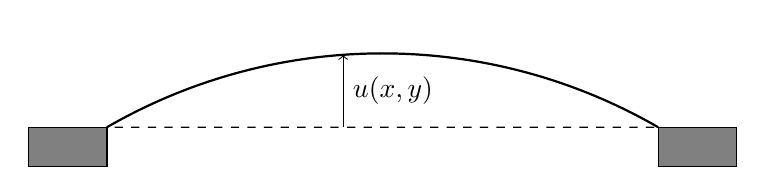
\begin{tikzpicture}

\draw [thick] (0,0) arc (120:60:7cm);
\draw (0,0) arc (120:60:7cm) [dashed] -- (0,0);

\draw [fill=gray] (0,0) rectangle ++(-1,-0.5);
\draw [fill=gray] (7,0) rectangle ++(1,-0.5);

\draw[->] (3,0) -- node[right]{$u(x,y)$} ++(0,0.92);

\end{tikzpicture}
\caption{A film of soapy water suspended across an aperture.}\label{soapy_c}
\end{figure}

\clearpage
Assume a pressure below the film distorts it, pushing it upwards.  If $f$ is the pressure, then the pressure force does work on the film equal to: $ W = \int_{\Omega} f u \,dA $.  The work done on the soap film is stored as elastic potential energy.  The soap film has a constant surface tension $k$ that acts tangentially to the surface.  The change in potential energy is proportional to the change in surface area, specifically $ U = k \frac{1}{2} \int_{\Omega} |\nabla u|^2 \;dA $.
A summary schematic is shown in Figure (\ref{balance_c}).

\begin{figure}[ht]
\centering
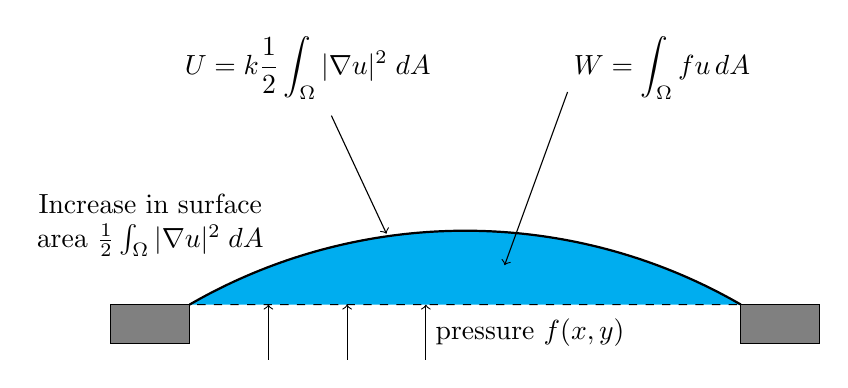
\begin{tikzpicture}

\draw [fill=cyan] (0,0) arc (120:60:7cm) [dashed] -- (0,0);
\draw [thick] (0,0) arc (120:60:7cm);

\draw [fill=gray] (0,0) rectangle ++(-1,-0.5);
\draw [fill=gray] (7,0) rectangle ++(1,-0.5);

\draw[<-] (3,0) -- node[right]{pressure $f(x,y)$} ++(0,-0.7);
\draw[<-] (1,0) -- ++(0,-0.7);
\draw[<-] (2,0) -- ++(0,-0.7);

\draw[<-] (4,0.5) -- ++(0.8,2.2);
\node at (6,3) {$\displaystyle W = \int_{\Omega} f u \,dA $};

\draw[<-] (2.5,0.9) -- ++(-0.7,1.5);
\node at (1.5,3) {$\displaystyle U = k \frac{1}{2} \int_{\Omega}  |\nabla u|^2 \;dA  $};

\renewcommand{\baselinestretch}{1.00}
\node at (-0.5,1)[align=center] {Increase in surface\\ area $ \frac{1}{2} \int_{\Omega}  |\nabla u|^2 \;dA $ };

\end{tikzpicture}
\caption{The work done distorting the soap film is equal to the elastic potential energy due to the increase in area.}\label{balance_c}
\end{figure}

%\textbf{NOTE:}  This also models the energy balance of a deformed rubber membrane, \emph{if} the deformation is small enough that the tension is considered to be \emph{constant} throughout the deformation (rather than increasing linearly with area).
The elastic potential energy is exactly equal to the work done on the soap film by the pressure:
\begin{equation}
k \frac{1}{2} \int_{\Omega} |\nabla u|^2 \;dA = \int_{\Omega} f u \;dA
\end{equation}
We can express this as a functional to be minimized:
\begin{equation}
F(u) =  k \frac{1}{2} \int_{\Omega} |\nabla u|^2 \,dA - \int_{\Omega} f u \,dA
\end{equation}
And take the functional derivative:                  
\begin{align}
\frac{d}{d\epsilon}F & = \lim_{\epsilon \rightarrow 0}
                         \frac{F(u + \epsilon v) - F(u)}{\epsilon} \\
  & =
    k \int_{\Omega} \nabla u \cdot \nabla v \,dA
        - \int_{\Omega} f v \,dA     
\end{align}
Thus the variational form $\frac{d}{d\epsilon}F = 0$ is:
\begin{equation}
k \int_{\Omega} \nabla u \cdot \nabla v \,dA
        - \int_{\Omega} f v \,dA = 0
\end{equation}
This relation is true for any \emph{almost} arbitrary variation $v$.  In fact, $v$ must be integrable on the domain $\Omega$, and its first derivatives must be integrable on $\Omega$.
The space of functions meeting these requirements is known as the Sobolev space $H^1(\Omega) $.  So formally, $v$ belongs to the Sobolev space:
\begin{equation}
v \in H^1 (\Omega)
\end{equation}
Moreover, because the value of $u$ is given at the boundary, $v$ must be zero at the boundary.  Formally, $v$ is in the Sobolev space:
\begin{equation}
v \in H_0^1 (\Omega)
\end{equation}

\section{Alternative Route to Variational Form}

The point is that the variational form
\begin{equation}
k \int_{\Omega} \nabla u \cdot \nabla v \,dA  - \int_{\Omega} f v \,dA = 0
\qquad
\forall v \in H_0^1(\Omega)
\end{equation}
may be easier to solve than the original energy functional:
\begin{equation}
k \frac{1}{2} \int_{\Omega} |\nabla u|^2 \,dA - \int_{\Omega} f u \,dA = 0
\end{equation}
However, the variational form can be derived by other means.  In fact, there are variational formulations for which there is \emph{no} corresponding functional to minimize.  So in a sense the variational formulation is more fundamental than the calculus of variations.

To illustrate:  The functional $ \frac{1}{2} \int_{\Omega} |\nabla u|^2 \,dA $ 
is known as Dirichlet's energy functional.  A solution $u$ that minimizes the functional is \emph{also} a solution to the Laplace equation $ \nabla^2 u = 0 $.
This energy functional can be put into the variational form $ \int_{\Omega} \nabla u \cdot \nabla v \,dA $ by using the calculus of variations.  However, the variational form $ \int_{\Omega} \nabla u \cdot \nabla v \,dA $ can also be derived directly from the Laplace equation.
\begin{equation}
u \; \text{minimizing} \;\;\; \frac{1}{2} \int_{\Omega} |\nabla u|^2 \,dA
\;\;\; \text{also satisfies} \;\; \int_{\Omega} \nabla u \cdot \nabla v \,dA = 0
\;\;\; \text{iff} \;\;\; \nabla^2 u =0 
\end{equation}

We shall use this alternative derivation as part of our homogenization procedure.
We bootstrap by building up from simpler cases:  First, we derive the variational form $ - \int_{\Omega} \nabla u \cdot \nabla g \,dA = \int_{\Omega} g f \,dA $ directly from the Poisson equation $ \nabla^2 u = f$, which we can think of as the $x$ velocity equation of Stokes flow with the pressure gradient given as (scalar) $f$.

Note on notation:  In an integral such as $ \int_{\Omega} g f \,dA $, the integration measure $dA$ is implied by the subscript $\Omega$ denoting integration over the domain.  Therefore, to improve readability -- without loss of clarity -- we shall usually drop the integration measures (such as $dA$) from the integrals.

\subsection{Variational Form of Poisson Equation inspired by Stokes Flow}

Here we derive the variational form $ - \int_{\Omega} \nabla u \cdot \nabla g = \int_{\Omega} g f $ directly from the Poisson equation $ \nabla^2 u = f$.  This is the $x$ velocity equation of Stokes flow with the pressure gradient given as scalar $f$, and the no-slip boundary condition.

Before beginning, we recall a vector identity.  For scalars $g$ and $u$:
% "Too much detail.  Your examiners can do this in their heads..."
%\begin{align*}
%g \nabla^2 u & = g \partial_x^2 u + g \partial_y^2 u \\
%\nabla u \cdot \nabla g & = \partial_x u \partial_x g + \partial_y u \partial_y g \\
%\nabla \cdot (g \nabla u) & = \partial_x (g \partial_x u) + \partial_y (g \partial_y u) \\
%  & = \partial_x u \partial_x g + g \partial_x^2 u + \partial_y u \partial_y g + g \partial_y^2 u \\ 
%  & = \nabla u \cdot \nabla g + g \nabla^2 u 
%\end{align*}
\begin{equation}
%\therefore \quad 
g \nabla^2 u = \nabla \cdot (g \nabla u) - \nabla u \cdot \nabla g
\end{equation}

\vspace{2em}

On some domain $\Omega$, as in Figure (\ref{domain}), the Poisson equation holds:
\begin{equation}
\nabla^2 u = f \qquad \text{on} \; \Omega
\end{equation}

\vspace{1em}
\begin{figure}[ht]
\centering
\begin{tikzpicture}
\draw[dashed] (0,0) rectangle (4,2);

\node at (2,1) {$\Omega $};
\node at (4.5,1) {$\Gamma $};
\end{tikzpicture}
\caption{A domain $\Omega$ with boundary $\Gamma$.}\label{domain}
\end{figure}

\clearpage
We introduce a \emph{test function} $g$, from the appropriate Sobolev space:  $g$ and its first derivatives are integrable on $\Omega$, and $g$ is zero on the boundary $\Gamma$:
\begin{equation}
g \in H_0^1(\Omega) \qquad (g=0 \; \text{on} \; \Gamma)
\end{equation}

We multiply the Poisson equation by the test function $g$:
\begin{equation}
g \nabla^2 u = g f
\end{equation}
and integrate over the domain $\Omega$:
\begin{equation}
\int_{\Omega} g \nabla^2 u = \int_{\Omega} g f
\end{equation}
then substitute $g \nabla^2 u = \nabla \cdot (g \nabla u) - \nabla u \cdot \nabla g$:
%\begin{equation}
%\int_{\Omega} \nabla \cdot (g \nabla u) - \nabla u \cdot \nabla g  
%= \int_{\Omega} g \nabla p
%\end{equation}
\begin{equation}
\int_{\Omega} \nabla \cdot (g \nabla u) - \int_{\Omega} \nabla u \cdot \nabla g  
= \int_{\Omega} g f
\label{eq:poissint}
\end{equation}

\begin{equation}
\text{Recall the Divergence Theorem:} \qquad
\int_{\Omega} \nabla \cdot \vec{a}  = \int_{\Gamma} \vec{a} \cdot \vec{n}
\end{equation}
Therefore the first term of Eq. (\ref{eq:poissint}) is:
\begin{equation}
\int_{\Omega} \nabla \cdot (g \nabla u) = 
\int_{\Gamma} (g \nabla u) \cdot \vec{n} = \int_{\Gamma} g (\nabla u \cdot \vec{n})
= \int_{\Gamma} g \frac{\partial u}{\partial n}
\end{equation}
Now the test function $g$ was defined to be zero on $\Gamma$, thus
\begin{equation}
\int_{\Omega} \nabla \cdot (g \nabla u)
 = \int_{\Gamma} g \frac{\partial u}{\partial n} =0
\end{equation}

This leaves finally:
\begin{equation}
- \int_{\Omega} \nabla u \cdot \nabla g  
= \int_{\Omega} g f
\end{equation}
which closely resembles the variational form derived from the energy functional.


\subsection{Variational Form of Poisson Equation inspired by Stokes Flow with Slip}

We now progress to the variational form of the Poisson equation inspired by Stokes flow over a flat boundary with Navier slip.

On the domain $\Omega$, the Poisson equation holds:
\begin{equation}
\nabla^2 u = f \qquad \text{on} \; \Omega
\end{equation}

Now the boundary of the entire domain, $\Gamma$, must be split up into the \emph{bottom} boundary $\Gamma_b$, and the rest of the boundary, $\Gamma_0$, as shown in Figure (\ref{splitboundary}).  The bottom boundary $\Gamma_b$ is the solid surface with slip.  The boundary condition on $\Gamma_b$ has the form of Navier slip:
\begin{equation}
u = b \frac{\partial u}{\partial n} \qquad \text{on} \; \Gamma_b
\end{equation}

\vspace{1em}
\begin{figure}[ht]
\centering
\begin{tikzpicture}
\draw (0,0) -- (4,0);
\draw[dashed] (0,0) -- ++(0,2) -| (4,0);

\node at (2,1) {$\Omega $};
\node at (2,-0.5) {$\Gamma_b$};
\node at (4.5,1) {$\Gamma_0 $};
\end{tikzpicture}
\caption{Domain $\Omega$ with slip boundary $\Gamma_b $ and remainder of boundary $\Gamma_0 $.}\label{splitboundary}
\end{figure}


Now care must be taken to choose the appropriate function space for our test function.  As before, the  test function and its first derivatives must be integrable on $\Omega$.  
But now, $g$ must vanish on all of the boundary \emph{except} the bottom boundary $\Gamma_b$:

\begin{equation}
g \in H^1_{\Gamma_b} (\Omega) = \lbrace g \in H^1(\Omega): g = 0 \; \text{on}\; \Gamma_0 \rbrace 
\quad (g \neq 0 \; \text{on} \; \Gamma_b)
\end{equation}

Multiply  by $g$ and integrate over $\Omega$:
\begin{equation}
\int_{\Omega} g \nabla^2 u = \int_{\Omega} g f
\end{equation}

Ending up with
\begin{equation}
\int_{\Gamma} g \frac{\partial u}{\partial n}
 - \int_{\Omega} \nabla u \cdot \nabla g  
= \int_{\Omega} g f
\end{equation}
Now, $g=0$ on all of $\Gamma$ except the bottom boundary, so:
\begin{equation}
\int_{\Gamma} g \frac{\partial u}{\partial n}
= \int_{\Gamma_b} g \frac{\partial u}{\partial n}
\end{equation}
The slip condition on $\Gamma_b$ implies:
\begin{equation}
\frac{\partial u}{\partial n} = \frac{1}{b}u
\end{equation}
So we substitute this, to get our variational form:
\begin{equation}
\int_{\Gamma_b} g \frac{1}{b} u 
 - \int_{\Omega} \nabla u \cdot \nabla g  
= \int_{\Omega} g f
\end{equation}

\clearpage
\section{Variational Form of Stokes Flow with\\ Tensor Slip}

\subsection{Tensor Identities}

Before deriving the variational formulation of our full model of 3-D flow with tensorial slip, we define the tensor double dot product and recall a tensor identity.

\subsubsection{Tensor Double Dot Product}

The double dot product of two tensors, also known as the Frobenius inner product, is a generalization of the vector inner product:

\begin{equation}
A = 
\begin{bmatrix}
a & b \\
c & d
\end{bmatrix}
, \quad Z = 
\begin{bmatrix}
x & y \\
z & w
\end{bmatrix}
, \quad
A:Z = ax + by + cz + dw
\end{equation}

\subsubsection{Tensor Identity with Deformation Rate Tensor}

In Appendix E, we prove the following identity:
\begin{equation}
\nabla^2 \vec{u} \cdot \vec{g} = 
\nabla \cdot ( (\nabla \vec{u} + \nabla \vec{u}^T) \cdot \vec{g})
- 2 \mathbf{E}(\vec{u}):\mathbf{E}(\vec{g})
\label{tensoridentity}
\end{equation}
This identity assumes $\nabla \cdot \vec{u} = 0$.

\clearpage
\subsection{Variational Form of Stokes Flow with Tensor Slip}

We have a domain $\Omega$, the boundary of which is made up of two parts, $\Gamma_b$ and $\Gamma_0$, as shown in Figure (\ref{Stokesdomain}).  On the domain $\Omega$ we have incompressible Stokes flow:
\begin{gather}
\nabla^2 \vec{u} = \frac{1}{\mu} \nabla p  \\
\nabla \cdot \vec{u} = 0
\end{gather}
On the rough boundary $\Gamma_b$ we have the tensor slip condition:
\begin{equation}
\frac{1}{b} \vec{u} = (\nabla \vec{u} + \nabla \vec{u}^T)\cdot \vec{n}
\quad \text{or} \quad
\frac{1}{b} \vec{u} = 2 \mathbf{E}(\vec{u}) \cdot \vec{n}
\label{tensorslipBC}
\end{equation}

\begin{figure}[ht]
\centering
\begin{tikzpicture}

\draw [domain=0:4.5,samples=200] plot (\x,{ 0.2 * sin(7*\x r)} );
\draw[dashed] (0,0) -- ++(0,2) -| (4.5,0);

\node at (2.25,-0.5) {$\Gamma_b $};
\node at (5,1) {$\Gamma_0 $};
\node at (2.25,1) {$\Omega $};

\end{tikzpicture}
\caption{Domain $\Omega$ with rough slip boundary $ \Gamma_b $ and remainder of boundary $\Gamma_0$.}\label{Stokesdomain}
\end{figure}

We introduce an arbitrary test function $\vec{g}$ from the appropriate Sobolev space:
\begin{equation}
\vec{g} \in H^1_{\Gamma_b}(\Omega) = 
\{ \vec{g} \in H^1(\Omega), \quad \nabla \cdot \vec{g} = 0 \text{ in } \Omega ,
 \quad \vec{g}=0 \text{ on } \Gamma_0 \}
\end{equation}

We take the dot product of the Stokes PDE with $\vec{g}$:
\begin{equation}
\nabla^2 \vec{u} \cdot \vec{g} = \frac{1}{\mu} \nabla p \cdot \vec{g}
\end{equation}
and integrate over the domain:
\begin{equation}
\int_{\Omega} \nabla^2 \vec{u} \cdot \vec{g} = 
\frac{1}{\mu} \int_{\Omega}  \nabla p \cdot \vec{g}
\end{equation}

%%%%
%Consider the right hand side.  Recall that by integration by parts:
%\begin{equation}
%\frac{1}{\mu} \int_{\Omega}  \nabla p \cdot \vec{g} = 
%\frac{1}{\mu} \int_{\Omega} \nabla \cdot p\vec{g} - 
%\frac{1}{\mu} \int_{\Omega} p \nabla \cdot \vec{g}
%\end{equation}
%By the Divergence Theorem:
%\begin{equation}
%\frac{1}{\mu} \int_{\Omega} \nabla \cdot p\vec{g} =
%\frac{1}{\mu} \int_{\Gamma} p \vec{g} \cdot \vec{n} =
%\frac{1}{\mu} \int_{\Gamma_b} p \vec{g} \cdot \vec{n} +
%\frac{1}{\mu} \int_{\Gamma_0} p \vec{g} \cdot \vec{n}
%\end{equation}


%Thus we have
%\begin{equation}
%\int_{\Omega} \nabla^2 \vec{u} \cdot \vec{g} = 
%\frac{1}{\mu} \int_{\Omega}  \nabla p \cdot \vec{g}
%\end{equation}

Substitute  $ \nabla^2 \vec{u} \cdot \vec{g} = \nabla \cdot ( 2 \mathbf{E}(\vec{u}) \cdot \vec{g}) - 2 \mathbf{E}(\vec{u}):\mathbf{E}(\vec{g}) $, (the tensor identity Equation (\ref{tensoridentity})):
\begin{equation}
\int_{\Omega} \nabla \cdot ( 2 \mathbf{E}(\vec{u}) \cdot \vec{g} ) - 
2 \int_{\Omega} \mathbf{E}(\vec{u}) : \mathbf{E}(\vec{g})  = 
\frac{1}{\mu} \int_{\Omega}  \nabla p \cdot \vec{g}
\end{equation}

By the Divergence Theorem:
\begin{equation}
\int_{\Omega} \nabla \cdot ( 2 \mathbf{E}(\vec{u}) \cdot \vec{g} ) =
\int_{\Gamma} ( 2 \mathbf{E}(\vec{u}) \cdot \vec{g} ) \cdot \vec{n}
\end{equation}
And $\mathbf{E}$ is symmetric, so:
\begin{equation}
\int_{\Gamma} ( 2 \mathbf{E}(\vec{u}) \cdot \vec{g} ) \cdot \vec{n} =
\int_{\Gamma} ( 2 \mathbf{E}(\vec{u})^T \cdot \vec{n} ) \cdot \vec{g} =
\int_{\Gamma} ( 2 \mathbf{E}(\vec{u}) \cdot \vec{n} ) \cdot \vec{g}
\end{equation}
The boundary integral can be split into separate integrals over $\Gamma_b$ and $\Gamma_0$.\begin{equation}
\int_{\Gamma} ( 2 \mathbf{E}(\vec{u}) \cdot \vec{n} ) \cdot \vec{g} =
\int_{\Gamma_b} ( 2 \mathbf{E}(\vec{u}) \cdot \vec{n} ) \cdot \vec{g} +
\int_{\Gamma_0} ( 2 \mathbf{E}(\vec{u}) \cdot \vec{n} ) \cdot \vec{g}
\end{equation}
Now, $\vec{g} = 0$ on $\Gamma_0$, so $ \int_{\Gamma_0} ( 2 \mathbf{E}(\vec{u}) \cdot \vec{n} ) \cdot \vec{g} $ vanishes.

While on $\Gamma_b$, the slip condition holds.
So we substitute the tensor slip boundary condition $ 2 \mathbf{E}(\vec{u}) \cdot \vec{n} = \frac{1}{b} \vec{u}$, (Equation (\ref{tensorslipBC})):
\begin{equation}
\int_{\Gamma_b} ( 2 \mathbf{E}(\vec{u}) \cdot \vec{n} ) \cdot \vec{g} =
\int_{\Gamma_b} \frac{1}{b} \vec{u} \cdot \vec{g}
\end{equation}
Therefore:
\begin{equation}
\int_{\Gamma} ( 2 \mathbf{E}(\vec{u}) \cdot \vec{n} ) \cdot \vec{g} =
\int_{\Gamma} \frac{1}{b} \vec{u} \cdot \vec{g}
\end{equation}
Thus:
\begin{equation}
\int_{\Omega} \nabla \cdot ( 2 \mathbf{E}(\vec{u}) \cdot \vec{g} ) =
\int_{\Gamma} \frac{1}{b} \vec{u} \cdot \vec{g}
\end{equation}

\vspace*{1em}
Hence the variational formulation for Stokes flow with tensor slip is:
\begin{equation}
\int_{\Gamma} \frac{1}{b} \vec{u} \cdot \vec{g} = 
2 \int_{\Omega} \mathbf{E}(\vec{u}) : \mathbf{E}(\vec{g}) +
\frac{1}{\mu} \int_{\Omega}  \nabla p \cdot \vec{g}
\end{equation}


\section{Weak Convergence}

Homogenizing our variational formulation involves setting up sequences of functions, taking the limits of those sequences, and exploiting the fact that periodic functions weakly converge to their mean.  Therefore, in this section, we explain the types of sequences we shall use, and give an explanation of weak convergence.

\subsection{Sequence of Functions}

Consider a function, say $f(x) = \sin(x)$, with an additional parameter $n$, where $n$ is a positive integer.  For example:
\begin{equation}
f_n = \frac{1}{n} \sin (x)
\label{eq:sineseq}
\end{equation}
For each $n \in \mathbb{Z}$ we have a new function.  Thus we have a \emph{sequence} of functions, indexed by $n$.  The first three are shown in Figure (\ref{sinesequence}).

\begin{figure}[ht]
\centering
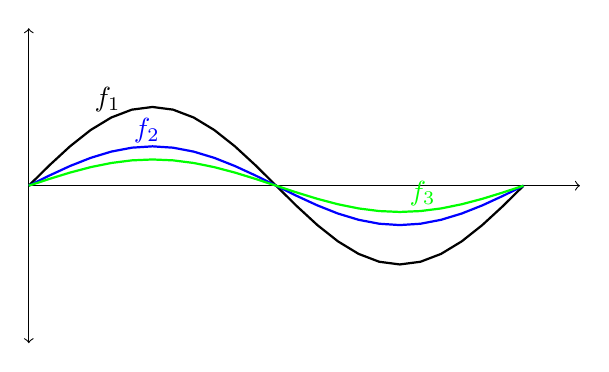
\begin{tikzpicture}

\draw[->] (0,0) -- (7,0);
\draw[<->] (0,-2) -- (0,2);

\draw [thick, domain=0:6.283] plot (\x, { sin(\x  r) });
\draw [color=blue,thick, domain=0:6.283] plot (\x, { sin(\x  r)/2 });
\draw [color=green,thick, domain=0:6.283] plot (\x, { sin(\x  r)/3 });

\node at (1,1.1) {$f_1$};
\node at (1.5,0.7) [color=blue] {$f_2$};
\node at (5,-0.1) [color=green] {$f_3$};

%\draw[color=red,thick, samples=97, domain=1:5] plot (\x, { 0.2 * sin( 3*pi*(\x-1) r) } );

\end{tikzpicture}
\caption{The first 3 functions of the sequence defined in Equation (\ref{eq:sineseq}).}\label{sinesequence}
\end{figure}

As $n \rightarrow \infty$, a sequence of functions may converge to a limit. (Or not.)
A function $f_n$ in the sequence may be made arbitrarily `close to' the limit function, by simply making $n$ large enough. (All subsequent functions after $f_n$ are at least as close.)

The functions, and the limit function, are points in a function space.  We need to define a `distance' between two points, that is, the notion of a function being `close to' another function.

\subsection{Strong Convergence}

In a vector space, the distance between two points $\vec{a}$ and $\vec{b}$ is found by finding the difference vector $\vec{b} - \vec{a}$, and calculating its length, the norm 
\begin{equation}
\lVert  \vec{b} - \vec{a} \rVert = \sqrt{(\vec{b} - \vec{a})\cdot (\vec{b} - \vec{a})}
\end{equation}
How do we extend this simple Pythagorean calculation to vectors of \emph{infinite} dimension? For the components $a_i$ of an infinite-dimensional vector, the index $i$ has an infinite domain, so the components can be thought of as a function $a(i)$ on a continuum. So the dot product $\vec{a} \cdot \vec{a}$ naturally extends to become the square integral:
\begin{equation}
\text{Inner Product } \vec{a} \cdot \vec{a} = \int \lvert a(x) \rvert^2 \;dx,
\quad \text{Norm } \lVert \vec{a} \rVert = \sqrt{\vec{a} \cdot \vec{a} }
\end{equation}

Coming from the other direction, the space of functions now has a natural inner product: $ \langle a,b \rangle = \int f \bar{g}\; dx $ which for $\langle a,a \rangle$ is the same as the square integral above.

The space of functions that are square-integrable, together with the inner product defined above, is the Lebesgue space $L^2$.  Our sequence of functions naturally live in this space.  We now have a natural notion of the `closeness' of a function to another: roughly speaking, the area \emph{between} the functions.

The sequence of functions \textbf{strongly converges} to the limit function $f$ if:
\begin{equation}
\lVert f_n - f \rVert \to 0 \qquad \text{as} \qquad n \to \infty
\end{equation}
Explicitly:
\begin{equation}
\int \lvert f_n - f \rvert^2 \;dx  \to 0 \qquad \text{as} \qquad n \to \infty
\end{equation}
This is notated:
\begin{equation}
f_n \to f
\end{equation}


\clearpage
\subsection{Weak Convergence}

Consider a sequence of functions defined by:
\begin{equation}
f_n = \sin(n x)
\end{equation}
the first three functions of which appear in Figure (\ref{sinnx_c}).
\begin{figure}[ht]
\centering
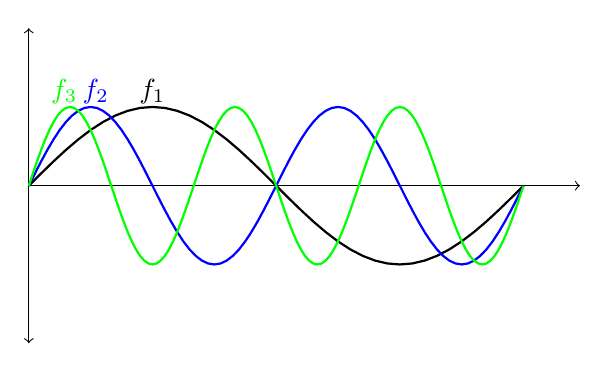
\begin{tikzpicture}

\draw[->] (0,0) -- (7,0);
\draw[<->] (0,-2) -- (0,2);

% samples = 4n per period + 1. n is resolution
\draw [thick, domain=0:6.283,samples=41] plot (\x, { sin(\x  r) });
\draw [color=blue,thick, domain=0:6.283, samples=81] plot (\x, { sin(2*\x  r) });
\draw [color=green,thick, domain=0:6.283, samples=121] plot (\x, { sin(3*\x r) });

\node at (1.57,1.2) {$f_1$};
\node at (0.85,1.2) [color=blue] {$f_2$};
\node at (0.45,1.2) [color=green] {$f_3$};

%\draw[color=red,thick, samples=97, domain=1:5] plot (\x, { 0.2 * sin( 3*pi*(\x-1) r) } );

\end{tikzpicture}
\caption{The first three functions in the sequence $\sin (n x)$.}\label{sinnx_c}
\end{figure}

As $n$ increases, the period of the sine wave gets smaller and smaller, but the amplitude is unchanged.  In the limit as $n \to \infty$, the waveform gets infinitely `spiky'.  What does the sequence converge to?  There is no intuitive sense of the sinewave sequence getting `closer to' some limit function.  In fact, the sequence does not strongly converge.

However, there is a sense in which the function sequence converges. 

We multiply each function in the sequence by an arbitrary test function $g$, and integrate, thus creating a sequence of integrals:
\begin{equation}
\int g f_n \;dx
\end{equation}
If the sequence of integrals (strongly) converges to a limit integral:
\begin{equation}
\int g f_n \;dx \to \int g f \;dx
\end{equation}
then we say that $f_n$ \textbf{weakly converges} to $f$, and the `limit function' $f$ appearing in the limit integral is known as the \textbf{weak limit.}  This is also written:
\begin{equation}
f_n \rightharpoonup f
\end{equation}

What is the weak limit $f$?  If $f_n$ is a sequence of periodic functions (like our sine wave example) then $f$ is the \textbf{mean} of $f_n$, denoted $\left< f_n \right>  $.

%We shall prove (and use) this incredibly useful result.

\subsection{Periodic Functions Weakly Converge to their Mean}

It is a `standard result' that periodic functions weakly converge to their mean.  In a 2002 paper \cite{Lukkassen2002}, Lukkassen and Wall state: ``We have not found proofs of [this] fact in the literature.  The aim of this paper is to present such proofs."  Their paper provides a rigorous proof (and generalization) of this proof.  In Appendix F, however, we present a simple intuitive proof, suitable for this thesis.

We show that periodic functions weakly converge to their mean:
\begin{equation}
\int g f_n \;dx \to \int g \left< f \right> \;dx
\end{equation}
We shall use this incredibly useful result to homogenize our variational form.


\clearpage
\section{Homogenizing the Variational Form}

Our variational form:
\begin{equation}
\int_{\Gamma} \frac{1}{b} \vec{u} \cdot \vec{g} = 
2 \int_{\Omega} \mathbf{E}(\vec{u}) : \mathbf{E}(\vec{g}) +
\frac{1}{\mu} \int_{\Omega}  \nabla p \cdot \vec{g}
\label{eq:variationalform}
\end{equation}
can now be homogenized.  The homogenization procedure we shall employ embodies two key concepts.

The first key concept is to model the slip boundary as a periodic function, and to set up a sequence of such functions, thus creating a sequence of boundaries.
Each boundary corresponds to a domain, so there is a sequence of domains.  Equation (\ref{eq:variationalform}) holds on each domain, so we have a sequence of systems to solve, and therefore a sequence of velocity and pressure field solutions.
The $n$-th variational formulation (that holds on the $n$-th domain with $n$-th boundary) contains slip length function $b_n$ and is satisfied by velocity field $\vec{u}_n$ and pressure field $p_n$:
\begin{equation}
\int_{\Gamma_n} \frac{1}{b_n} \vec{u}_n \cdot \vec{g}_n = 
2 \int_{\Omega_n} \mathbf{E}(\vec{u}_n) : \mathbf{E}(\vec{g}_n) +
\frac{1}{\mu} \int_{\Omega_n}  \nabla p_n \cdot \vec{g}_n
\label{eq:nthvariationalform}
\end{equation}

The second key concept is to define the sequence such that it converges to a \emph{limit} system.  The idea is that while it may be difficult to solve any system in the sequence, the limit system is easy to solve.  We could define a sequence of boundaries such that the period and amplitude of the surface function halve with each increment of $n$.  We similarly reduce the period of the slip length function with each increment of $n$.  The amplitude of $b$ remains unchanged.  Then, the sequence of systems converges to a system with a flat plane boundary with a limiting slip length of the same order as that in the sequence systems.  The overall size $P$ of the domain also remains approximately constant for all $n$.  This is illustrated in Figure (\ref{domainseq}).


\clearpage
\begin{figure}[ht]
\centering
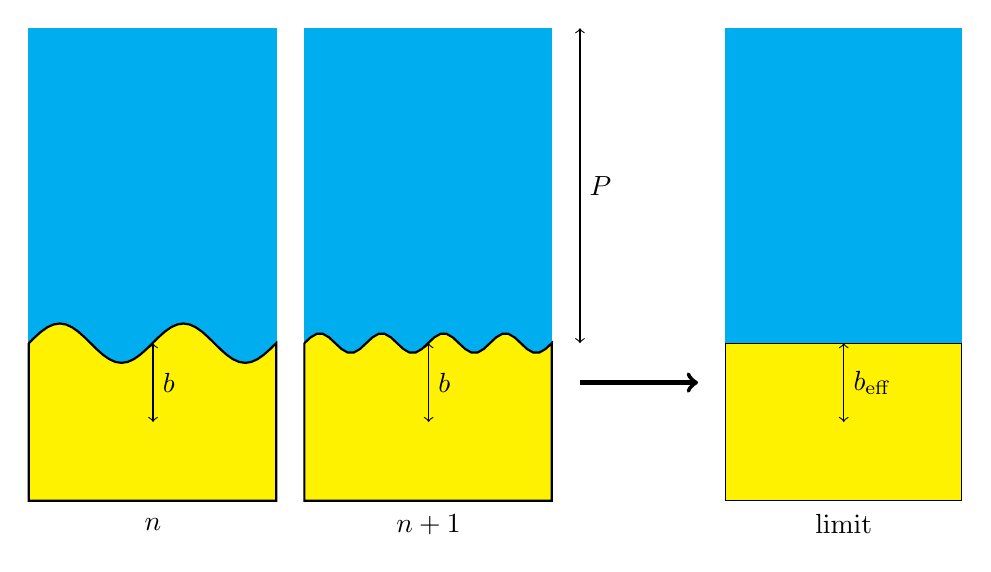
\begin{tikzpicture}
%\draw [thick, domain=0:6.283,samples=41] plot (\x, { sin(\x  r) });

\draw [fill=cyan,color=cyan] (0,-1) rectangle ++(3.1416, 5);
\draw [fill=cyan,color=cyan] (3.5,-1) rectangle ++(3.14, 5);
\draw [fill=cyan,color=cyan] (8.85,-1) rectangle ++(3, 5);



\draw [fill=yellow, thick, domain=0:3.1416,samples=41] plot (\x, { sin(4*\x  r)/4 })
 |- (0,-2) -- (0,0);

\draw [fill=yellow, thick, domain=0:3.1416,samples=41] plot (\x+3.5, { sin(8*\x  r)/8 })
 |- (3.5,-2) -- (3.5,0);

\draw[->, ultra thick] (7,-0.5) -- ++(1.5,0);

\draw[fill=yellow] (8.85,0) rectangle ++(3,-2);

\draw[<->](1.578,0) -- node[right]{$b$} ++(0,-1);
\draw[<->](5.078,0) -- node[right]{$b$} ++(0,-1);
\draw[<->](10.35,0) -- node[right]{$\beff$} ++(0,-1);

\node at (1.578,-2.3) {$n$};
\node at (5.078,-2.3) {$n+1$};
\node at (10.35,-2.3) {limit};

\draw[<->] (7,0) -- node[right]{$P$} ++(0,4);

\end{tikzpicture}
\caption{A sequence of domains, where the period and amplitude of the boundary halve with each increment of $n$, converging on a limit domain.}\label{domainseq}
\end{figure}



\subsubsection{Sequence of Boundaries}

The physical boundary is a periodic function $h(x,y)$.  (For simplicity we shall illustrate it as a sine function, but it need not be.)  
The slip length is a periodic function $b(x,y)$ with the \textbf{same period} as $h(x,y)$.

\vspace{1em}
Define a sequence of surface functions by:
\begin{equation}
h_n = \frac{1}{n} h(nx, ny)
\end{equation}
As $n \to \infty$, the amplitude of $h_n \to 0$.  This ensures convergence to a plane.
Similarly, define a sequence of slip functions by:
\begin{equation}
b_n = b(nx,ny)
\end{equation}
In this case, as $n$ increases, the period shortens, but the amplitude of $b_n$ does \textbf{not} decrease.
We have a sequence of boundaries $\Gamma_n$ that (strongly) converges to the flat $x,y$ plane, as shown in Figure (\ref{boundseq}).

\begin{figure}[ht]
\centering
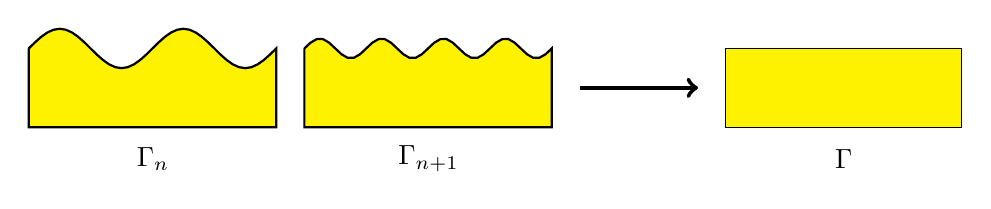
\begin{tikzpicture}
%\draw [thick, domain=0:6.283,samples=41] plot (\x, { sin(\x  r) });

\draw [fill=yellow, thick, domain=0:3.1416,samples=41] plot (\x, { sin(4*\x  r)/4 })
 |- (0,-1) -- (0,0);

\draw [fill=yellow, thick, domain=0:3.1416,samples=41] plot (\x+3.5, { sin(8*\x  r)/8 })
 |- (3.5,-1) -- (3.5,0);

\draw[->, ultra thick] (7,-0.5) -- ++(1.5,0);

\draw[fill=yellow] (8.85,0) rectangle ++(3,-1);

\node at (1.578,-1.4) {$\Gamma_n$};
\node at (5.078,-1.4) {$\Gamma_{n+1}$};
\node at (10.35,-1.4) {$\Gamma$};

\end{tikzpicture}
\caption{The sequence of boundaries converges to the flat $x,y$ plane.}\label{boundseq}
\end{figure}


\subsubsection{Sequence of Gradient Functions}

Consider our definition of the sequence of surfaces: $ h_n = \frac{1}{n} h(nx, ny) $.
As $n$ increases, the period and amplitude reduce by the \textbf{same factor.}  This means that for a point on the surface at a given fraction of the period, the slope at that point does not change with $n$. 
This is best explained by example.  If the the base function is simple sinusoids in $x$ and $y$: $h(x,y) = \sin(x)\sin(y)$, then
\begin{equation}
h_n = \frac{1}{n} \sin(nx)\sin(ny) \quad \Rightarrow \quad
\begin{cases}
\partial_x h_n = \cos(nx)\sin(ny) \\ \partial_y h_n = \cos(ny)\sin(nx)
\end{cases}
\label{eq:slopeconstant}
\end{equation}
Clearly, the amplitudes of $\nabla h_n = (\partial_x h_n, \partial_y h_n)$ over one period do not change with increasing $n$.  However, with increasing $n$, the period reduces, leading to a more and more `spiky' function.
As shown in Appendix F, such a sequence of functions weakly converges to its mean.

%Let $L_n$ be the period of surface function $h_n$, and $x_n$ the $x$ variable in domain $\Omega_n$.  Then:
%\begin{equation}
%\frac{x_i}{L_i} = \frac{x_j}{L_j} \Rightarrow 
%h_i' \left( \frac{x_i}{L_i} \right) = h_j' \left( \frac{x_j}{L_j} \right)
%\label{eq:slopeconstant}
%\end{equation}
%Then the gradient $\nabla h$ will not `blow up' with increasing $n$.


%This is physically correct -- the local slip length is an intrinsic property of the material, unaffected by scale.


\subsubsection{Slip Integral}

Let us look more closely at the integral containing the slip length term, on the left-hand-side of Equation (\ref{eq:variationalform}).  The integral is over a surface; each infinitesimal area element $dA$ is the area of the tangent plane to $h(x,y)$. Specifically:
\begin{equation}
dA = \sqrt{1 + \lvert \nabla h \rvert^2} \;dxdy
\end{equation}
Furthermore, the velocity function on the boundary is $\vec{u}(x,y,h)$.  Similarly, for the test function $\vec{g}(x,y,h)$.
Therefore, the slip integral is explicitly:
\begin{equation}
\int_{\Gamma} \frac{1}{b} \vec{u} \cdot \vec{g} \;dA =
\int_{\Gamma} \frac{1}{b(x,y)} \vec{u}(x,y,h) \cdot \vec{g}(x,y,h) 
\;\sqrt{1 + \lvert \nabla h \rvert^2} \;dxdy
\end{equation}
%We insert the boundary sequence into the slip integral, giving:
%\begin{equation}
%\int_{\Gamma_n} \frac{\sqrt{1 + \lvert \nabla h_n \rvert^2}}{b_n} \;
% \vec{u}(x,y,h_n) \cdot \vec{g}(x,y,h_n) \;dxdy
%\end{equation}
%We now have a sequence of integrals.  This implies that we have a sequence of velocity fields $\vec{u}_n$ that satisfy these equations.  Therefore the sequence of integrals showing the explicit $n$-dependence of each term is:
For the $n$-th domain in the sequence, the slip integral is:
\begin{equation}
\int_{\Gamma_n} \frac{\sqrt{1 + \lvert \nabla h_n \rvert^2}}{b_n} \;
 \vec{u}_n(x,y,h_n) \cdot \vec{g}_n(x,y,h_n) \;dxdy
\end{equation}



%As summarised by Equation (\ref{eq:slopeconstant}), while $h_n$ converges to the flat plane, it is constructed such that its partial derivatives in $\nabla h_n$ remain unchanged with increasing $n$.
As illustrated by the example of Equation (\ref{eq:slopeconstant}), the magnitude of $\nabla h_n$ does not change with $n$.
Thus the the magnitude of $\sqrt{1 + \lvert \nabla h_n \rvert^2}$ does not change with increasing $n$. % --- the function simply gets `spikier' as the period reduces.
Furthermore, the slip function $b_n$ is constructed to exhibit the same behaviour: unchanging amplitude with decreasing period.
Therefore, the compound function $\sqrt{1 + \lvert \nabla h_n \rvert^2} /b_n$ exhibits this common behaviour, getting `spikier' with increasing $n$.
This type of sequence of functions weakly converges to its mean:
%As mentioned previously, these sorts of functions weakly converge to their mean:
\begin{equation}
\int_{\Gamma_n} \frac{\sqrt{1 + \lvert \nabla h_n \rvert^2}}{b_n} \;
\vec{g}_n\;dxdy \to
\int_{\Gamma} \left< \frac{\sqrt{1 + \lvert \nabla h \rvert^2}}{b} \right> \;
\vec{g} \;dxdy
\end{equation}
(Where the test function strongly converges: $ \vec{g}_n(x,y,h_n) \to \vec{g}(x,y,0) $.)

We add the velocity term $\vec{u}_n(x,y,h_n)$ to the above weak integral, to get the full slip integral.  
Since the boundary converges to the flat $x,y$ plane, we expect the velocity term to strongly converge to a single \emph{constant} velocity on the flat limit boundary:
\begin{equation}
\vec{u}_n(x,y,h_n) \to \vec{u}(x,y,0) \qquad \text{as} \quad n \to \infty
\end{equation}
Therefore, the integrand with the velocity term
 % still exhibits the `spiky' behaviour, and 
still weakly converges to its mean:
\begin{equation}
\int_{\Gamma_n} \frac{\sqrt{1 + \lvert \nabla h_n \rvert^2}}{b_n} \;
\vec{u}_n \cdot \vec{g}_n\;dxdy \to
\int_{\Gamma} \left< \frac{\sqrt{1 + \lvert \nabla h \rvert^2}}{b} \right> \;
\vec{u} \cdot \vec{g} \;dxdy
\end{equation}

\subsubsection{Sequence of Variational Formulations and its Limit}

%As the boundary changes, the domain $\Omega$ changes shape slightly also, giving a sequence of domains $\Omega_n$.  Therefore we have a sequence of volume integrals.  Thus, finally, we have a sequence of variational formulations:

Thus we have a sequence of variational formulations:
\begin{equation}
\int_{\Gamma_n} \frac{\sqrt{1 + \lvert \nabla h_n \rvert^2}}{b_n} \;
\vec{u}_n \cdot \vec{g}_n\;dxdy = 
2 \int_{\Omega_n} \mathbf{E}(\vec{u}_n) : \mathbf{E}(\vec{g}_n) +
\frac{1}{\mu} \int_{\Omega_n}  \nabla p_n \cdot \vec{g}_n
\end{equation}

which strongly converges to:
\begin{equation}
\int_{\Gamma} \left< \frac{\sqrt{1 + \lvert \nabla h \rvert^2}}{b} \right> \;
\vec{u} \cdot \vec{g} \;dxdy = 
2 \int_{\Omega} \mathbf{E}(\vec{u}) : \mathbf{E}(\vec{g}) +
\frac{1}{\mu} \int_{\Omega}  \nabla p \cdot \vec{g}
\label{eq:limitformulation}
\end{equation}


%Let us pause for a moment to gaze in awe at this limit variational formulation, and reflect on its significance.
%  By reversing the derivation shown earlier,
% we would arrive back at the classical formulation with


\subsection{Convert to Classical Formulation}
The limit variational formulation Equation (\ref{eq:limitformulation}) corresponds to the classical formulation with
\begin{equation}
\nabla^2 \vec{u} = \frac{1}{\mu} \nabla p
\end{equation}
on the domain, while on the boundary $\Gamma_b$ we would have the tensor slip condition:
\begin{equation}
\left< \frac{\sqrt{1 + \lvert \nabla h \rvert^2}}{b} \right> \vec{u} = 2 \mathbf{E}(\vec{u}) \cdot \vec{n}
\end{equation}

This slip boundary condition defines our effective slip length:
\begin{equation}
\beff = \left< \frac{\sqrt{1 + \lvert \nabla h \rvert^2}}{b} \right> ^{-1}
\label{eq:homogharm}
\end{equation}

This is the central result of this thesis.  It was published in 2012 \cite{Lund2012}.

\clearpage
\subsection{Interpretation}
We now discuss a physical interpretation of the result.
Note that the integral $\int_{\Omega} \sqrt{1 + \lvert \partial_x h \rvert^2} \; dx$ is the \textbf{arc length} of the function $h$ over the domain $\Omega$.  Extending to a three-dimensional surface,  $\int_{\Omega} \sqrt{1 + \lvert \nabla h \rvert^2} \; dxdy$ is the area of the surface function $h(x,y)$.

Hence, our effective slip is the \textbf{harmonic mean} of the local slip length, \textbf{weighted} by the fluid-solid contact area.  See Figure (\ref{contact}).

\begin{figure}[ht]
\centering
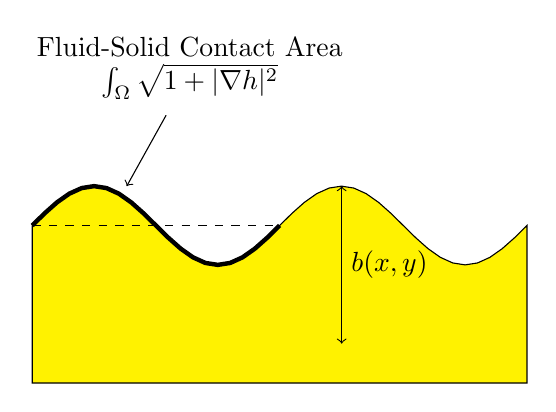
\begin{tikzpicture}

%samples = 4n per period + 1
\draw [fill=yellow, domain=0:6.283,samples=41] plot (\x, {sin(2*\x  r)/2 })
 |- ++(0,-2) -| (0,0); 
\draw [ultra thick, domain=0:3.1416,samples=21] plot (\x, {sin(2*\x  r)/2 });

\draw[dashed] (0,0) -- ++(3.1416,0);

\node at (2,2) [align=center]{Fluid-Solid Contact Area\\ $\int_{\Omega} \sqrt{1 + \lvert \nabla h \rvert^2} $};
\draw [<-] (1.2,0.5) -- ++(0.5,0.9);

\draw[<->] (3.93,0.5) -- node[right] {$b(x,y)$} ++(0,-2);

\end{tikzpicture}
\caption{$\beff$ incorporates the contact area between liquid and solid.}\label{contact}
\end{figure}

If the surface is flat, then $\beff$ is simply the harmonic mean of the intrinsic slip length:
\begin{equation}
\beff = \left< \frac{1}{b} \right> ^{-1}
\end{equation}

If the surface is a flat \textbf{binary} surface, comprising discrete areas of high-slip surface and low-slip surface, with high-slip regions occupying fraction $\phi$ of the surface, then:
\begin{equation}
\beff = \left[ \phi \frac{1}{ b_{\mathrm{high}} }  + (1 -\phi) \frac{1}{ b_{\mathrm{low}}} \right]^{-1}
\end{equation}
as first proposed by Cottin-Bizonne \emph{et al} in 2004 \cite{Cottin-Bizonne2004}.

\clearpage
\subsection{Applicability}

The effective slip length derived via homogenization is the \textbf{limiting} slip length as the period of the surface variation tends to zero.  A real surface obviously has a finite period of surface variation.  The effective slip length can in principle be measured experimentally.  

The critical question is:

\vspace{1em}
For what range of surfaces is the homogenized slip length a good approximation to the measured slip length?

\vspace{1em}
Equivalently, when is the flow over a rough, heterogeneous surface \textbf{close to} the flow over an effective homogenized surface?  

One approach to answer this is to ask: when is a rough surface close to the limit surface?  A reasonable answer is: when the \textbf{period is small compared to other length scales.}
There are two other length scales, the domain size $P$ and slip length $b$.  Therefore, we expect Equation (\ref{eq:homogharm}) to be a good approximation to measured slip length when:
\begin{equation}
L \ll b, P
\end{equation}
In our numerical testing (described in Chapter 8), we discover that our homogenized
effective slip length (Eq. (\ref{eq:homogharm})) is a surprisingly good approximation even when slip lengths are of the same order as the period:
\begin{equation}
L \sim b \ll P
\end{equation}


\iftoggle{compilealone}
    {
    \bibliography{Lund_Thesis.bib}
    \bibliographystyle{plain}
    }

\end{document}



There are two other length scales, the slip length $b$ and domain size $P$, with -- in general -- $b \ll P$.
%The only other length scale is the intrinsic slip length.  
Therefore, we propose that our $\beff$ is valid when the \textbf{minimum} intrinsic slip length is large compared to the period.

\begin{equation}
L \ll \bmin % \min(b(x,y))
\end{equation}

\clearpage
%In general, the condition $L \ll \bmin$ subsumes the requirement $L \ll P$.

Experimentally, $\beff$ is measured in the far field, where velocity is uniform and laminar, since the $x$-dependence found near the surface is smoothed out by velocity diffusion.  The notion of a `far field' at the top of the domain implies that $L \ll P$.

If $b \ll L$ on a surface, then the surface roughness would dominate the far-field $\beff$, with true slip length $b$ swamped by the roughness amplitude.
But if $b \sim L$ on a surface, then $b$ would feature significantly in the far-field $\beff$.  Therefore, we expect that if the intrinsic slip length has the same order of magnitude as the period, and the height $P$ of the far-field region is much bigger than $L$, then the homogenized $\beff$ would be a reasonable approximation to the $\beff$ measured in the far field.
\begin{equation}
b \sim L \ll P
\end{equation}
In practice -- specifically, in our numerical testing -- we find that our $\beff$ approximates the measured effective slip length very well when the minimum slip length is the same order of magnitude as the period.
(Details follow in Chapter \ref{C:numerics}.)% Chapter 8.




%\begin{center} \vspace{3em} \Coffeecup \end{center}

\iftoggle{compilealone}
    {
    \bibliography{Lund_Thesis.bib}
    \bibliographystyle{plain}
    }

\end{document}



